\documentclass{article}
\usepackage{graphicx} %package to manage images
\graphicspath{ {./figures/} }
\usepackage{hyperref}
\usepackage{caption}
\usepackage[font=scriptsize]{subcaption}
\captionsetup[figure]{labelsep=none}
\captionsetup[table]{labelsep=none}
\usepackage{bbm}
\usepackage{amsmath}
\usepackage{import}
\usepackage{array}
\usepackage{booktabs}
\usepackage{afterpage}
\usepackage{floatrow}
\usepackage{pdflscape}
\usepackage{soul}
\usepackage{float}
\usepackage{adjustbox}
\usepackage{longtable}


\title{trends in health in pregnancy (overleaf)}

\date{April 2025}

\begin{document}

\maketitle



TODO
- add short note after each figure/table and about how it was generated
\begin{figure}[H]
    \centering
    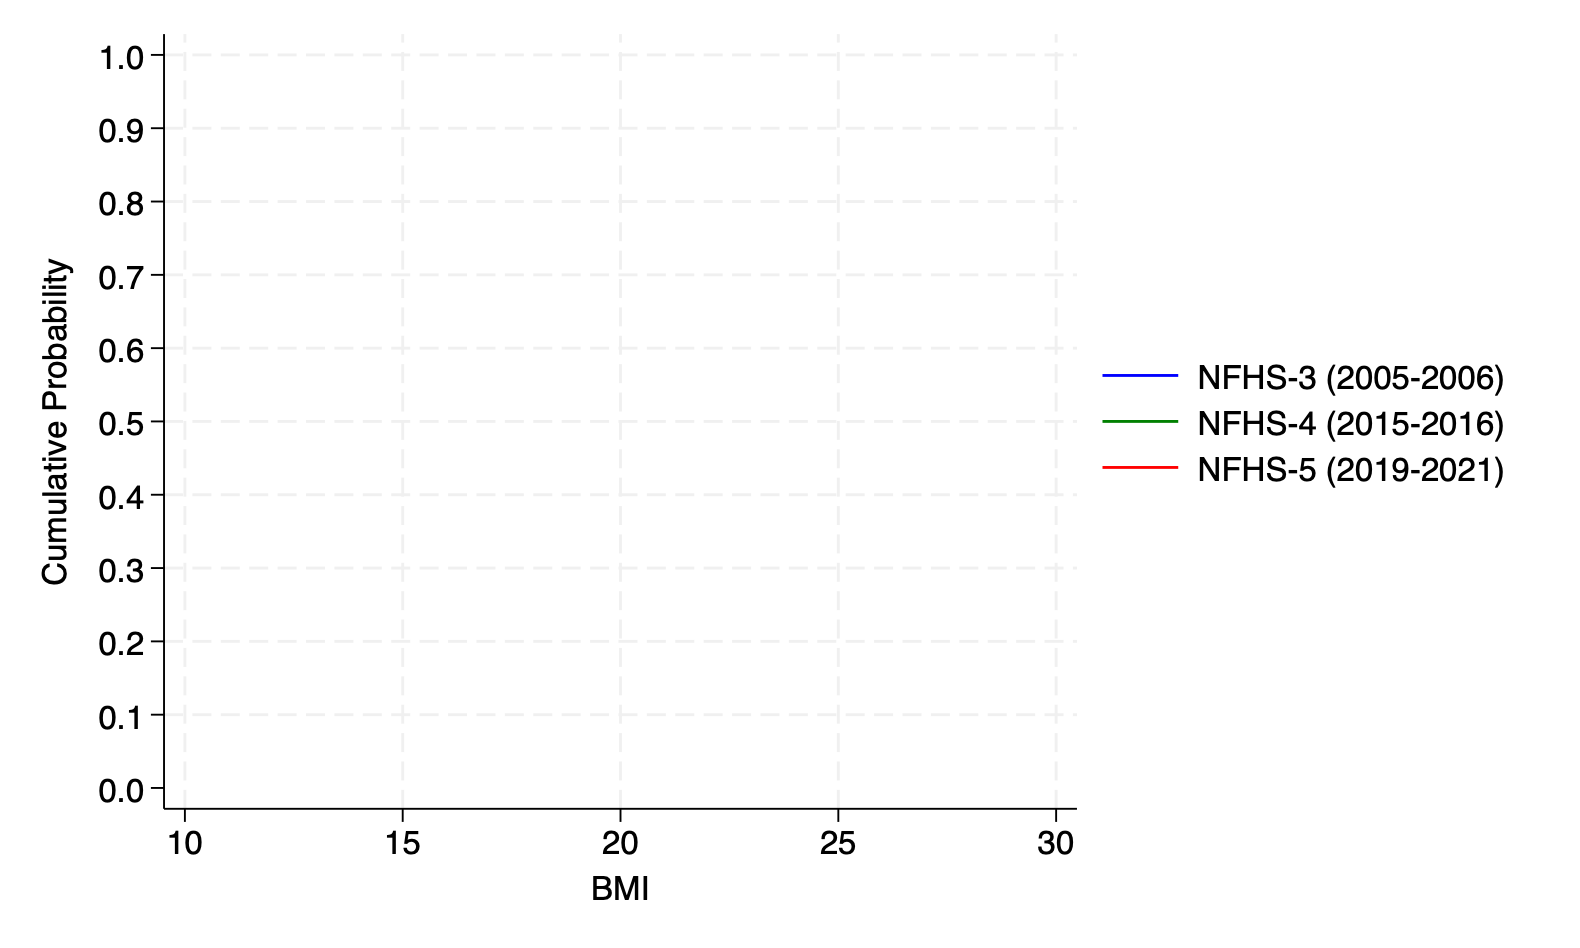
\includegraphics[width=\textwidth]{figures/cdf prepregnancy bmi.png}
    \caption{: CDFs of Estimated Pre-Pregnancy BMI in NFHS 3, 4, \& 5}
    
\end{figure}



\begin{figure}[H]
    \centering
    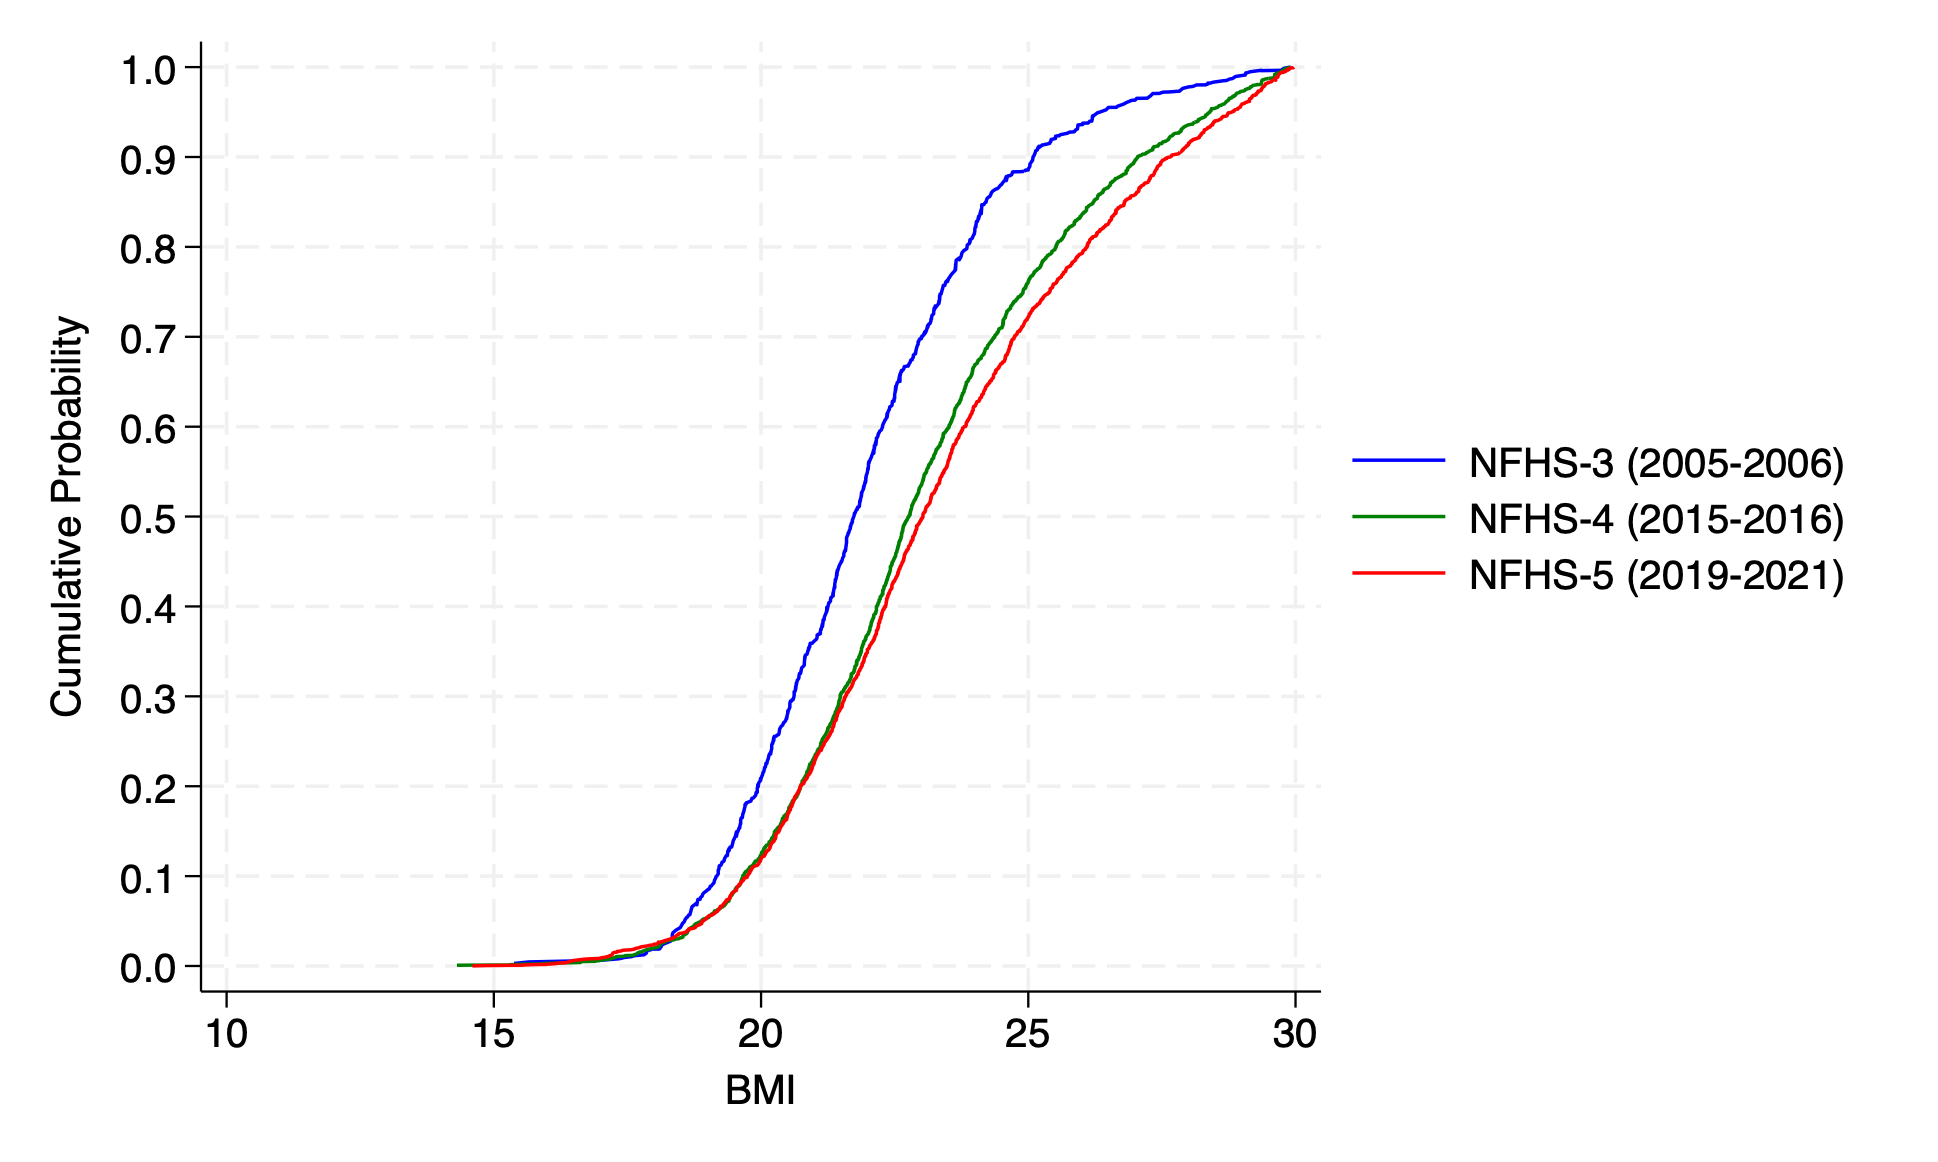
\includegraphics[width=\textwidth]{figures/cdf nine months bmi.png}
    \caption{: CDFs of Observed BMI at 9+ months pregnant in NFHS 3, 4, \& 5}
    
\end{figure}


\begin{figure}[H]
    \centering
    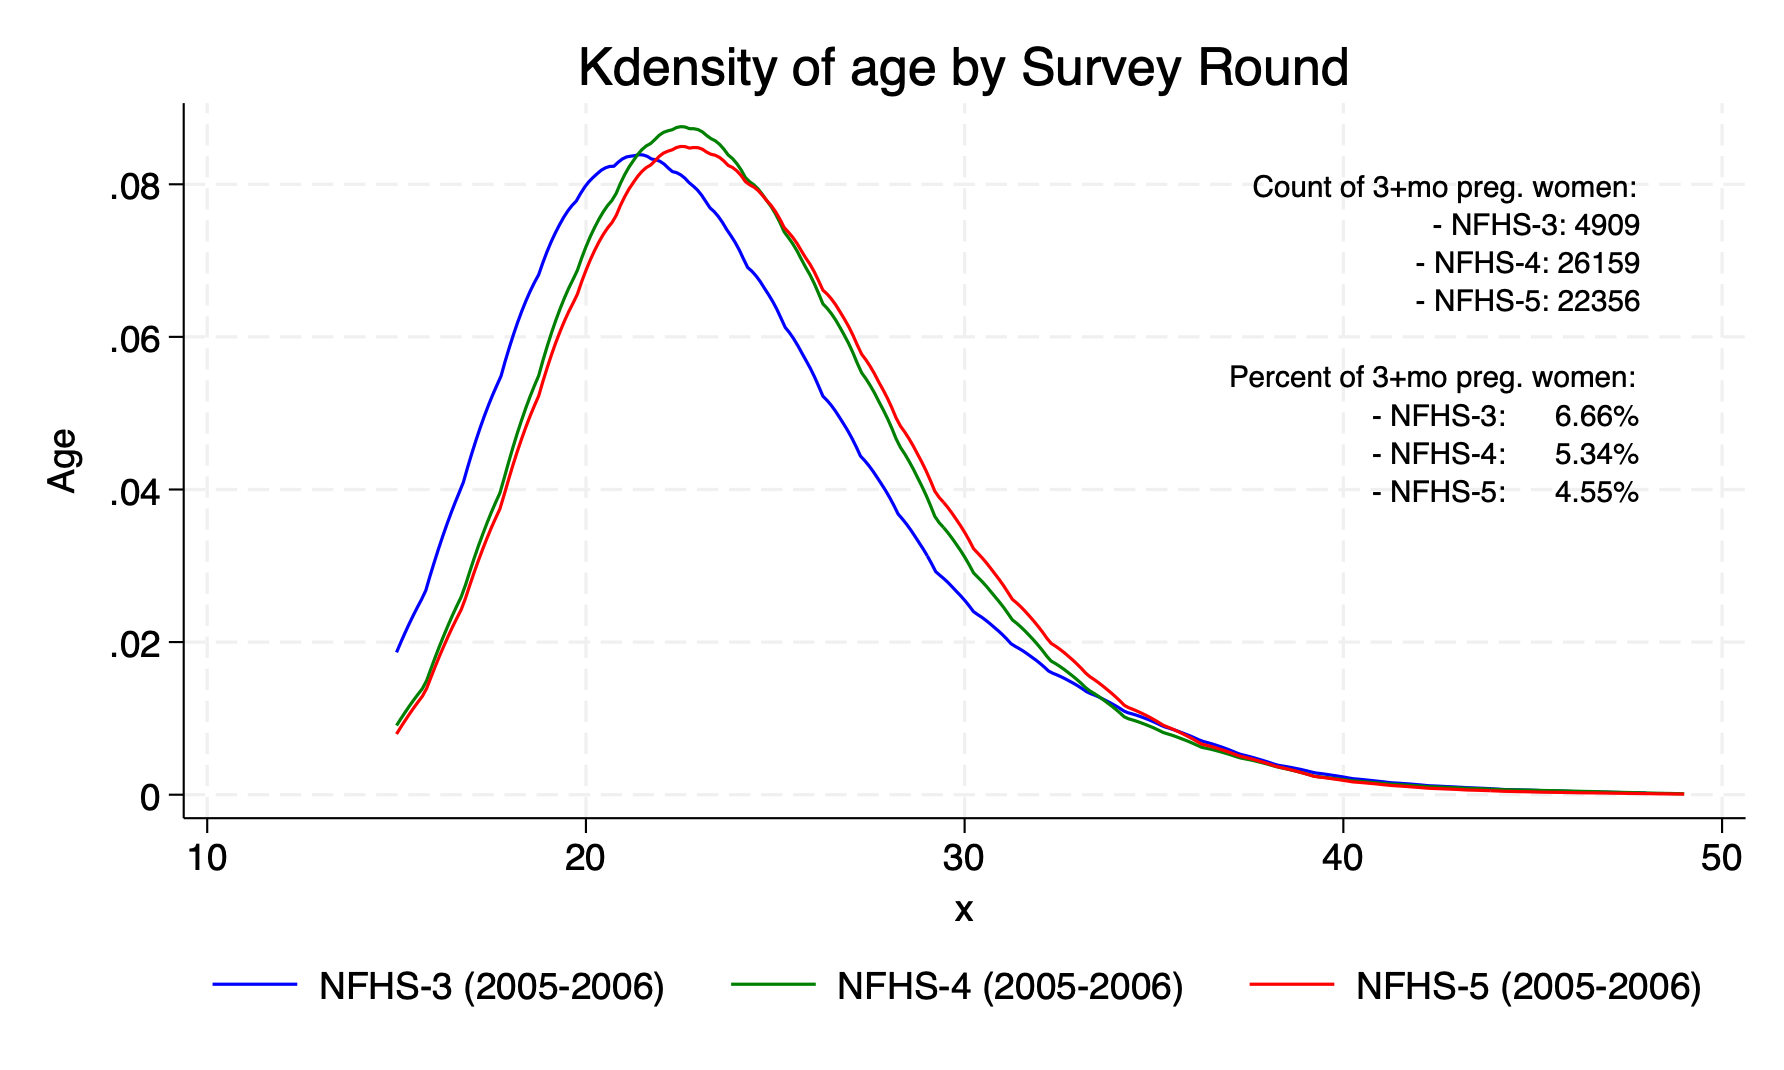
\includegraphics[width=\textwidth]{figures/kdensities ages.png}
    \caption{: Kernel density of the ages of currently pregnant women in NFHS 3, 4, \& 5}
\end{figure}


\begin{figure}[H]
    \centering
    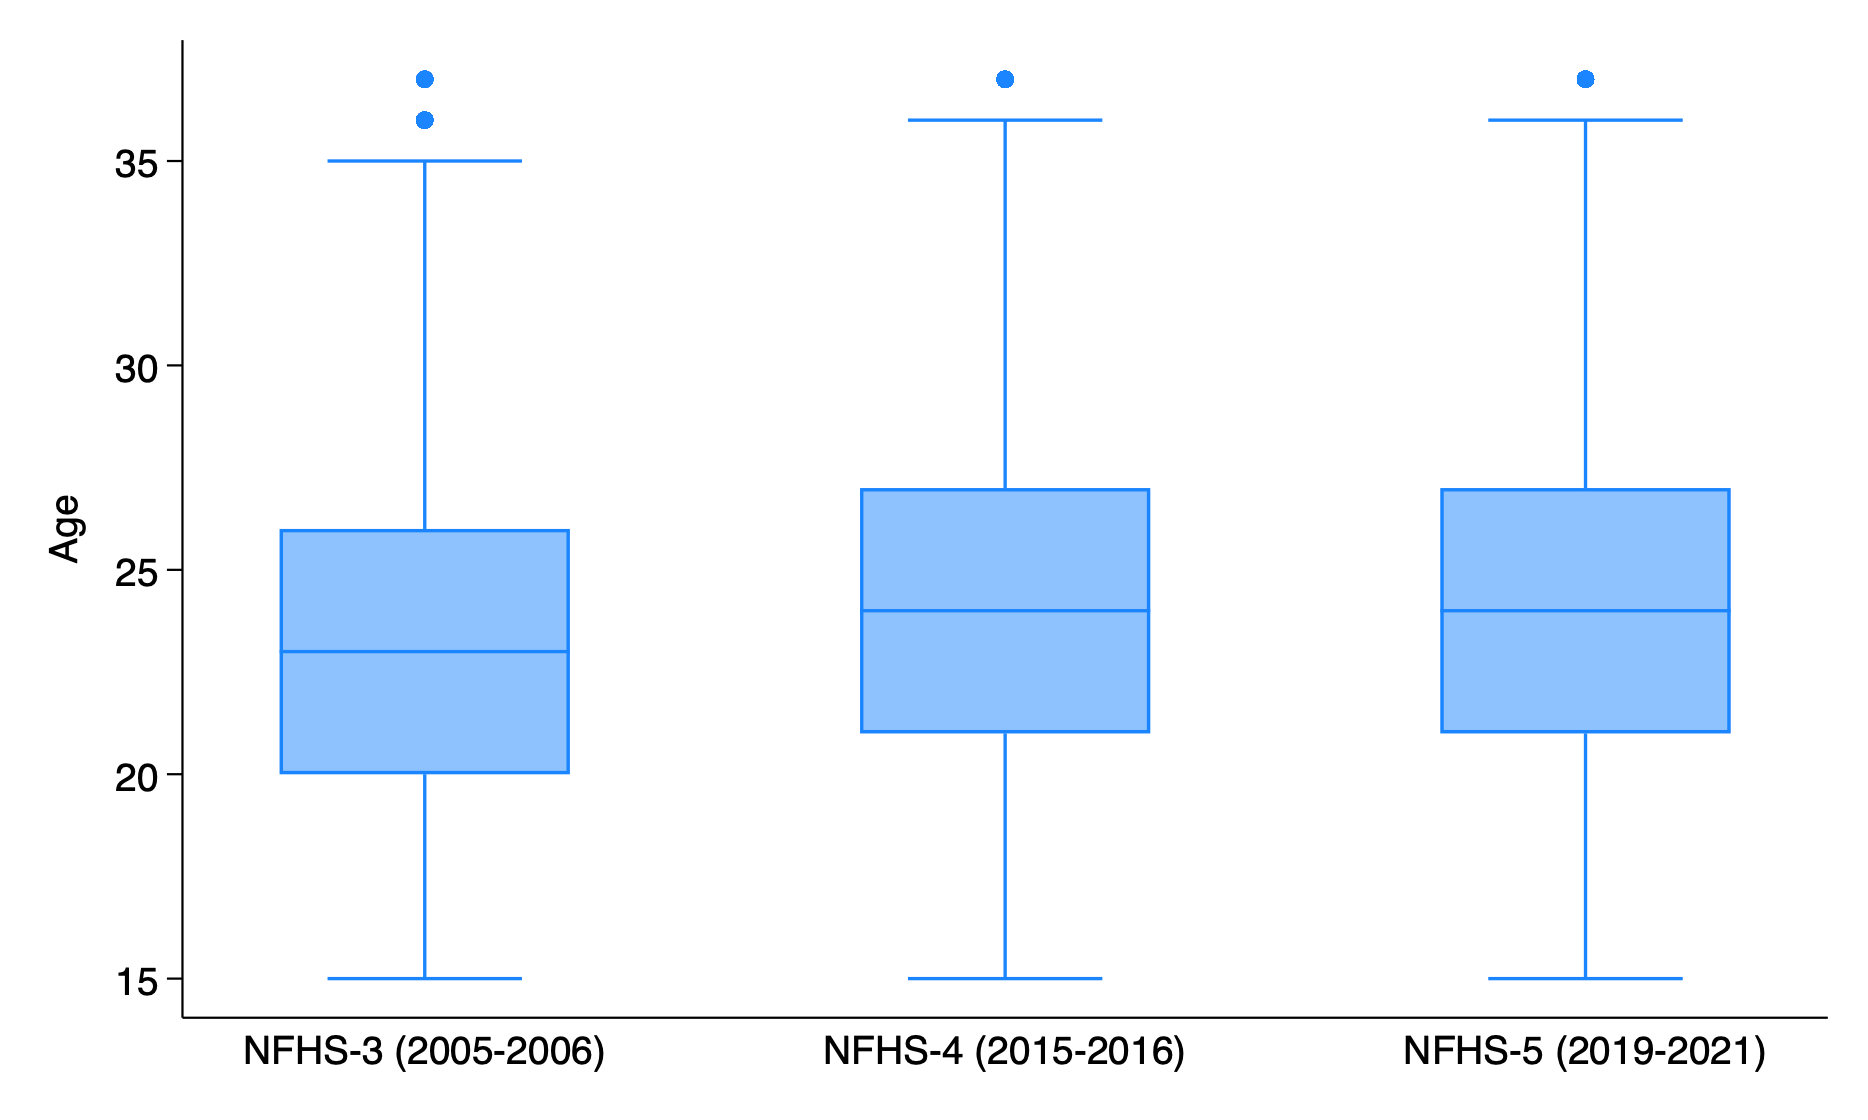
\includegraphics[width=\textwidth]{figures/boxplots ages.png}
    \caption{: Box plots of the age distributions of currently pregnant women NFHS 3, 4, \& 5}
\end{figure}

\begin{figure}[H]
    \centering
    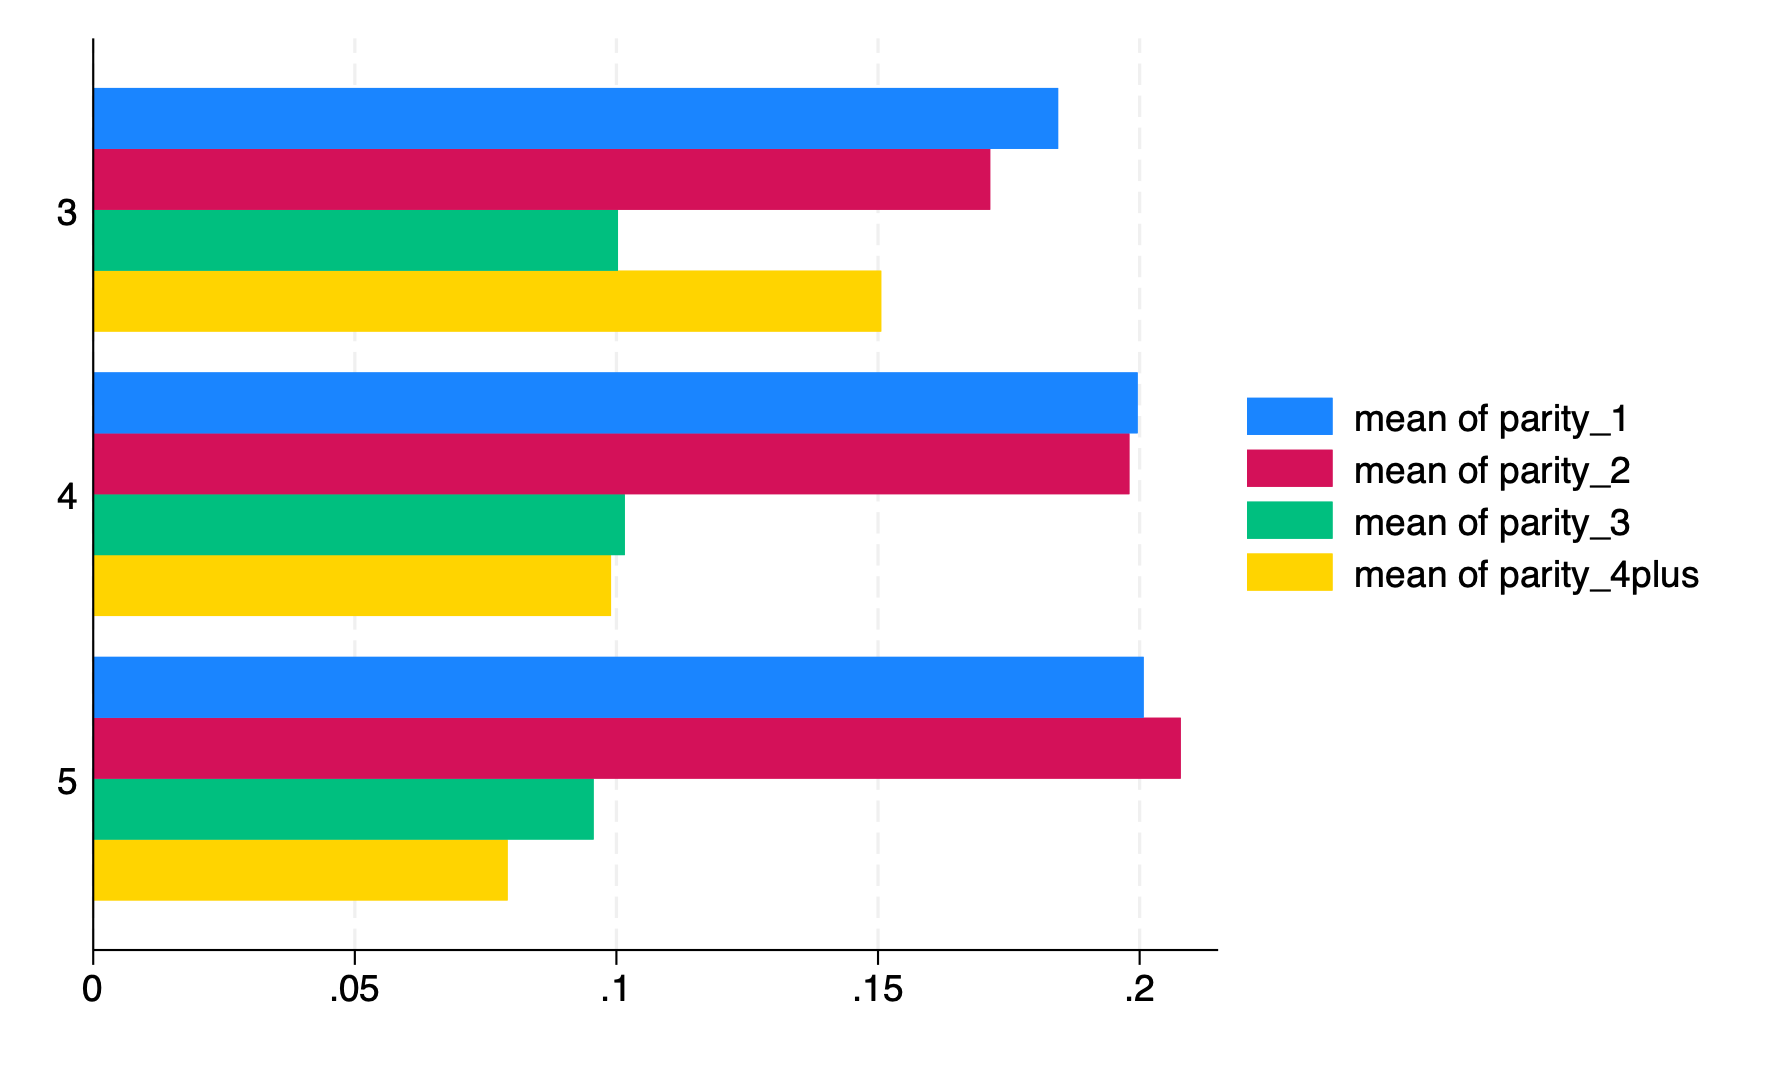
\includegraphics[width=\textwidth]{figures/bar graph number of children.png}
    \caption{: Bar graph of number of living children among currently pregnant women in the NFHS 3, 4, \& 5}
\end{figure}



\begin{table}[H]
    \centering
    \caption{: Proportion of pregnant women by gestational duration in the NFHS 3, 4, \& 5}
    \label{tab:sumstat}
    \adjustbox{width=\textwidth}{\begin{tabular}{l*{6}{c}}
\toprule
            &NFHS-3 (2005-2006)&            &NFHS-4 (2015-2016)&            &NFHS-5 (2019-2021)&            \\
            &\multicolumn{1}{c}{Mopreg}&\multicolumn{1}{c}{Moperiod}&\multicolumn{1}{c}{Mopreg}&\multicolumn{1}{c}{Moperiod}&\multicolumn{1}{c}{Mopreg}&\multicolumn{1}{c}{Moperiod}\\
\midrule
\midrule
1           &       1.807&       5.163&       4.602&       1.762&       4.987&       4.473\\
2           &       8.775&       8.199&       8.635&       8.696&       7.657&       8.285\\
3           &       13.44&       13.26&       12.38&       13.14&       12.51&       11.98\\
4           &       12.85&       12.83&       12.75&       12.74&       11.96&       12.37\\
5           &       12.73&       13.42&       12.21&       12.57&       12.60&       11.80\\
6           &       12.10&       12.19&       12.42&       11.86&       11.48&       11.82\\
7           &       11.84&       11.92&       12.00&       11.68&       11.20&       11.50\\
8           &       12.33&       12.02&       13.07&       12.14&       11.20&       12.26\\
9           &       11.28&       8.505&       9.477&       10.93&       7.918&       8.995\\
10          &       2.651&       2.060&       2.165&       2.638&       2.052&       2.144\\
11          &       0.196&       0.436&       0.277&       0.196&       0.436&       0.277\\
\bottomrule
\multicolumn{7}{l}{\footnotesize Mopreg refers to respondents self reported gestational duration. Moperiod refers months since last menstrual period.}\\
\end{tabular}
}
\end{table}



\begin{table}[H]
    \centering
    \caption{: Proportion of wanted pregnancies among pregnant women by parity in the NFHS 3, 4, \& 5}
    \label{tab:sumstat}
    \adjustbox{width=\textwidth}{{
\def\sym#1{\ifmmode^{#1}\else\(^{#1}\)\fi}
\begin{tabular}{l*{3}{c}}
\hline\hline
            &\multicolumn{1}{c}{NFHS-3}&\multicolumn{1}{c}{NFHS-4}&\multicolumn{1}{c}{NFHS-5}\\
\hline
\hline
Parity 1    &       85.14         &       94.99         &       94.85         \\
Parity 2    &       74.04         &       88.12         &       88.97         \\
Parity 3    &       71.06         &       80.72         &       81.92         \\
Parity 4+   &       55.21         &       69.60         &       74.63         \\
\hline\hline
\multicolumn{4}{l}{\footnotesize \textit{t} statistics in parentheses}\\
\multicolumn{4}{l}{\footnotesize \sym{*} \(p<0.05\), \sym{**} \(p<0.01\), \sym{***} \(p<0.001\)}\\
\end{tabular}
}
}
\end{table}


TODO: 
- make sure it's only non-pregnant women.
\begin{table}[H]
    \centering
    \caption{: Proportion of married women using modern contraception in the NFHS 3, 4, \& 5}
    \label{tab:sumstat}
    \adjustbox{width=\textwidth}{\begin{tabular}{l*{3}{c}}
\toprule
            &\multicolumn{1}{c}{NFHS-3 (2005–2006)}&\multicolumn{1}{c}{NFHS-4 (2015–2016)}&\multicolumn{1}{c}{NFHS-5 (2019–2021)}\\
\midrule
\midrule
No living boy child&       12.06&       15.33&       25.50\\
No children &       4.031&       6.664&       14.29\\
\bottomrule
\end{tabular}
}
\end{table}
Interpretation: women are more able to decide despite social pressure of having a boy/child

\begin{figure}[H]
    \centering
    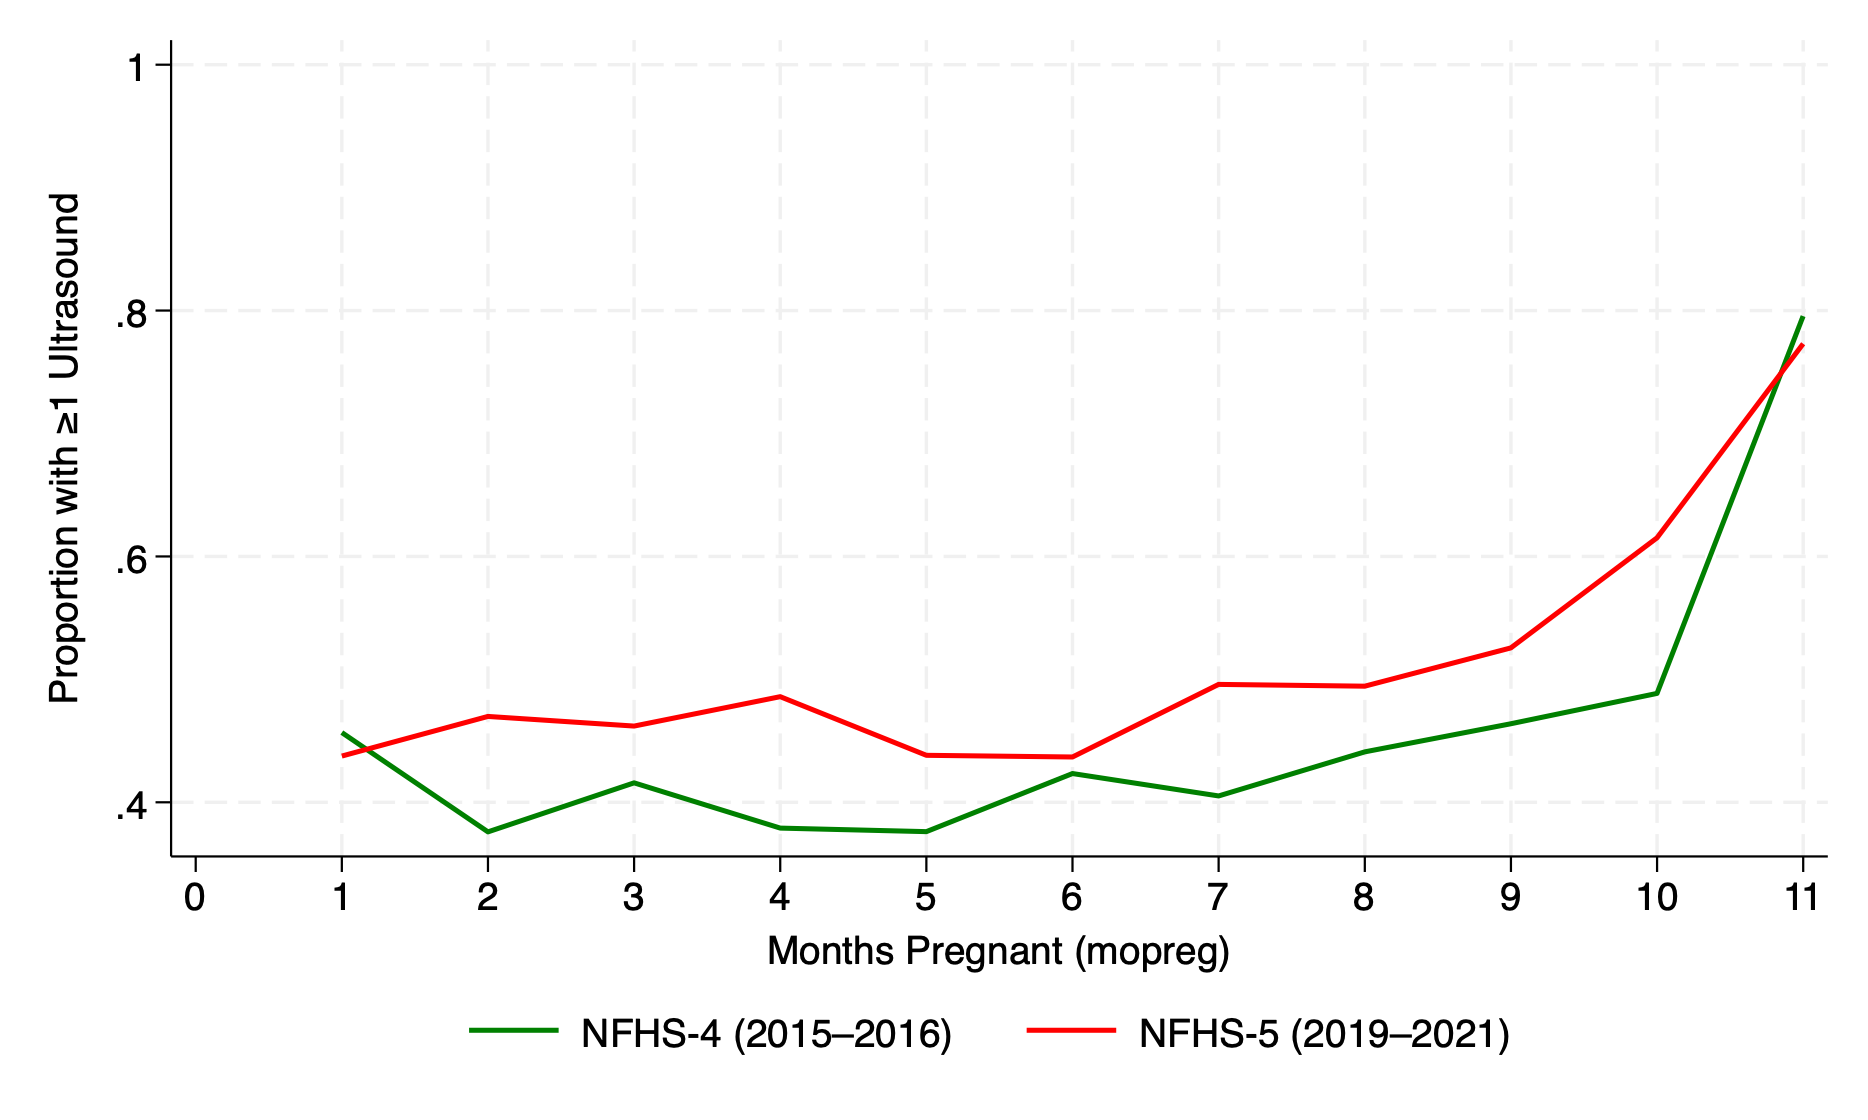
\includegraphics[width=\textwidth]{figures/ultrasound by pregnancy duration.png}
    \caption{: Proportion of pregnant women who have had an ultrasound by gestational duration in NFHS 4, \& 5}
\end{figure}




\begin{figure}[H]
    \centering
    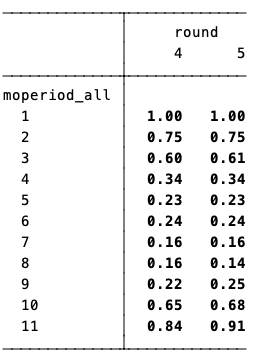
\includegraphics[width=\textwidth]{tables/says pregnant by gestational duration.png}
    \caption{: Proportion of women who report not being pregnant by months since last period in the NFHS 4, \& 5}
\end{figure}



\begin{table}[H]
    \centering
    \renewcommand{\arraystretch}{0.65} % shrink row height
    \setlength{\tabcolsep}{4pt} % shrink column padding
    \footnotesize % shrink text
    \caption{: Sample sizes table}
    \label{tab:sumstat}
    \begin{adjustbox}{width=\textwidth}
        {
\def\sym#1{\ifmmode^{#1}\else\(^{#1}\)\fi}
\begin{tabular}{l*{3}{ccc}}
\hline\hline
                    &      NFHS-3&            &            &      NFHS-4&            &            &      NFHS-5&            &            \\
                    &\multicolumn{3}{c}{}                  &\multicolumn{3}{c}{}                  &\multicolumn{3}{c}{}                  \\
                    &        Mean&          lb&          ub&        Mean&          lb&          ub&        Mean&          lb&          ub\\
\hline
eag                 &        0.56&      0.5450&      0.5704&        0.53&      0.5279&      0.5388&        0.54&      0.5297&      0.5413\\
north               &        0.12&      0.1164&      0.1333&        0.11&      0.1094&      0.1163&        0.13&      0.1300&      0.1380\\
central             &        0.28&      0.2733&      0.2964&        0.28&      0.2786&      0.2884&        0.27&      0.2621&      0.2724\\
east                &        0.27&      0.2613&      0.2841&        0.25&      0.2485&      0.2580&        0.27&      0.2631&      0.2734\\
northeast           &        0.04&      0.0329&      0.0427&        0.03&      0.0306&      0.0344&        0.04&      0.0393&      0.0440\\
Rural               &        0.75&      0.7410&      0.7631&        0.71&      0.7099&      0.7198&        0.74&      0.7389&      0.7491\\
Urban               &        0.25&      0.2369&      0.2590&        0.29&      0.2802&      0.2901&        0.26&      0.2509&      0.2611\\
Forward Caste       &        0.26&      0.2445&      0.2668&        0.20&      0.1915&      0.2002&        0.17&      0.1690&      0.1778\\
OBC                 &        0.42&      0.4040&      0.4292&        0.45&      0.4445&      0.4553&        0.44&      0.4356&      0.4472\\
Dalit               &        0.20&      0.1912&      0.2117&        0.22&      0.2125&      0.2214&        0.23&      0.2234&      0.2331\\
Adivasi             &        0.09&      0.0848&      0.0996&        0.10&      0.0924&      0.0988&        0.10&      0.0968&      0.1038\\
Muslim              &        0.18&      0.1691&      0.1887&        0.17&      0.1692&      0.1775&        0.17&      0.1686&      0.1774\\
Sikh/Jain/Christian &        0.03&      0.0260&      0.0347&        0.04&      0.0339&      0.0379&        0.03&      0.0321&      0.0364\\
Observed in nuclear family&        0.36&      0.3499&      0.3745&        0.29&      0.2831&      0.2930&        0.27&      0.2617&      0.2720\\
Observed in sasural &        0.45&      0.4336&      0.4590&        0.53&      0.5244&      0.5352&        0.55&      0.5472&      0.5588\\
Observed in meika   &        0.12&      0.1158&      0.1327&        0.13&      0.1225&      0.1297&        0.13&      0.1261&      0.1339\\
Observed in mother-in-law's home&        0.13&      0.1245&      0.1419&        0.16&      0.1511&      0.1590&        0.16&      0.1554&      0.1639\\
Observed in father-in-law's home&        0.34&      0.3264&      0.3506&        0.41&      0.4035&      0.4142&        0.42&      0.4185&      0.4300\\
bhai                &        0.31&      0.2959&      0.3195&        0.34&      0.3352&      0.3455&        0.33&      0.3210&      0.3319\\
bade\_bhai           &        0.00&      0.0024&      0.0056&        0.00&      0.0041&      0.0056&        0.01&      0.0049&      0.0067\\
chota\_bhai          &        0.03&      0.0300&      0.0393&        0.03&      0.0259&      0.0294&        0.02&      0.0185&      0.0218\\
bahu                &        0.37&      0.3590&      0.3837&        0.45&      0.4440&      0.4549&        0.48&      0.4743&      0.4860\\
mother              &        0.00&      0.0007&      0.0028&        0.00&      0.0008&      0.0016&        0.00&      0.0019&      0.0030\\
father              &        0.00&     -0.0001&      0.0009&        0.00&      0.0004&      0.0010&        0.00&      0.0002&      0.0007\\
Natal (usual residence)&        0.03&      0.0275&      0.0365&        0.05&      0.0514&      0.0563&        0.06&      0.0566&      0.0621\\
Natal (visiting)    &        0.09&      0.0849&      0.0997&        0.07&      0.0695&      0.0751&        0.07&      0.0676&      0.0736\\
Sasural – FIL present&        0.32&      0.3045&      0.3283&        0.38&      0.3720&      0.3825&        0.40&      0.3903&      0.4017\\
Sasural – MIL present&        0.11&      0.1010&      0.1170&        0.12&      0.1189&      0.1260&        0.13&      0.1257&      0.1335\\
Sasural – PILs present&        0.02&      0.0173&      0.0246&        0.03&      0.0282&      0.0320&        0.03&      0.0255&      0.0293\\
Nuclear HH – Woman is head&        0.03&      0.0285&      0.0377&        0.02&      0.0225&      0.0258&        0.03&      0.0298&      0.0339\\
Nuclear HH – Husband is head&        0.33&      0.3171&      0.3412&        0.26&      0.2591&      0.2687&        0.24&      0.2301&      0.2399\\
\hline
Observations        &        5867&            &            &       32401&            &            &       28350&            &            \\
\hline\hline
\end{tabular}
}

    \end{adjustbox}

\end{table}





\end{document}



fix lines on end-pregnancy BMI
remove titles on graphs from stata
label xaxis on kdensity age
maybe make stats on kdensity age separate table




- different living situations between pregnant, non-pregnant women (with reweighting), all non-pregnant women (without reweighting)
- create categories of household type accordingly
- model off: https://link.springer.com/article/10.1007/s13524-012-0173-1

- then get breakdown of proportion of pregnant



